\speaker{\Michel}

\begin{frame}
\frametitle{\underline{M}VC : Le modèle}
\begin{figure}[!h]
	\begin{center}
	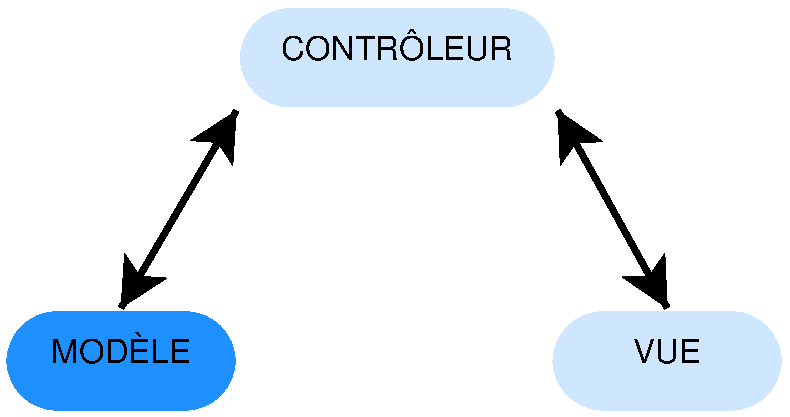
\includegraphics[scale=0.5]{images/mvcModele}
	\caption{Architecture \underline{M}VC}
	\end{center}
\end{figure}
\end{frame}

%%%%%%%%%%%%%%%%%%%%%%%%%%%%%%%%%%%%%%%%%%%%%%%%%%%

\begin{frame}
	\frametitle{\underline{M}VC : Le modèle}
	\begin{block}{Modélisation de la base de données}	
		\begin{itemize}
			\item Réalisation du diagramme de classes
			\item Création de la Base de Données et mapping avec les entités du projet
		\end{itemize}
	\end{block}
\end{frame}

%%%%%%%%%%%%%%%%%%%%%%%%%%%%%%%%%%%%%%%%%%%%%%%%%%%

\begin{frame}
	\frametitle{\underline{M}VC : Le modèle}
	\begin{block}{Création de la Base de Données et utilisation de l'ORM Doctrine}	
		\begin{columns}
			\begin{column}{0.9cm}
			\end{column}
			\begin{column}{6cm}
				\begin{Large} Top Down\end{Large}
				\begin{itemize}
					\item Approche descendante
					\item Système d'annotation dans les classes PHP
					\item Génération des tables de la Base de Données
				\end{itemize}
		\end{column}
		
		\begin{column}{4cm}
			\begin{figure}[!h]
				\begin{center}
					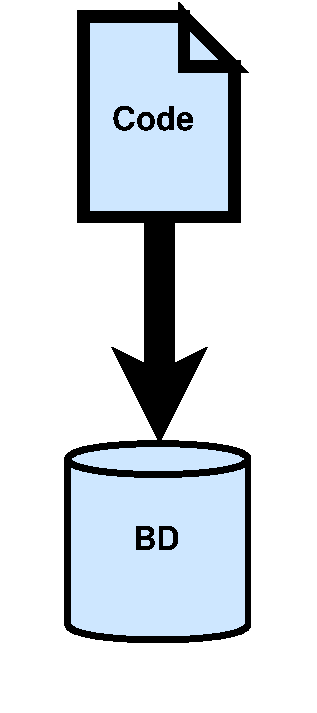
\includegraphics[scale=0.275]{images/topDown}
					\caption{Top Down}
				\end{center}
			\end{figure}
		\end{column}
	
	\end{columns}
	\end{block} 
\end{frame}

\begin{frame}
	\frametitle{\underline{M}VC : Le modèle}
	\begin{block}{Création de la Base de Données et utilisation de l'ORM Doctrine}	
		\begin{columns}
			\begin{column}{0.9cm}
			\end{column}
			\begin{column}{6cm}
				\begin{Large}Bottom Up\end{Large}
				\begin{itemize}
					\item Approche ascendante
					\item Création de la Base de Données
					\item Génération des fichiers de mapping et classes PHP
				\end{itemize}
			\end{column}
			
			\begin{column}{4cm}
			\begin{figure}[!h]
				\begin{center}
					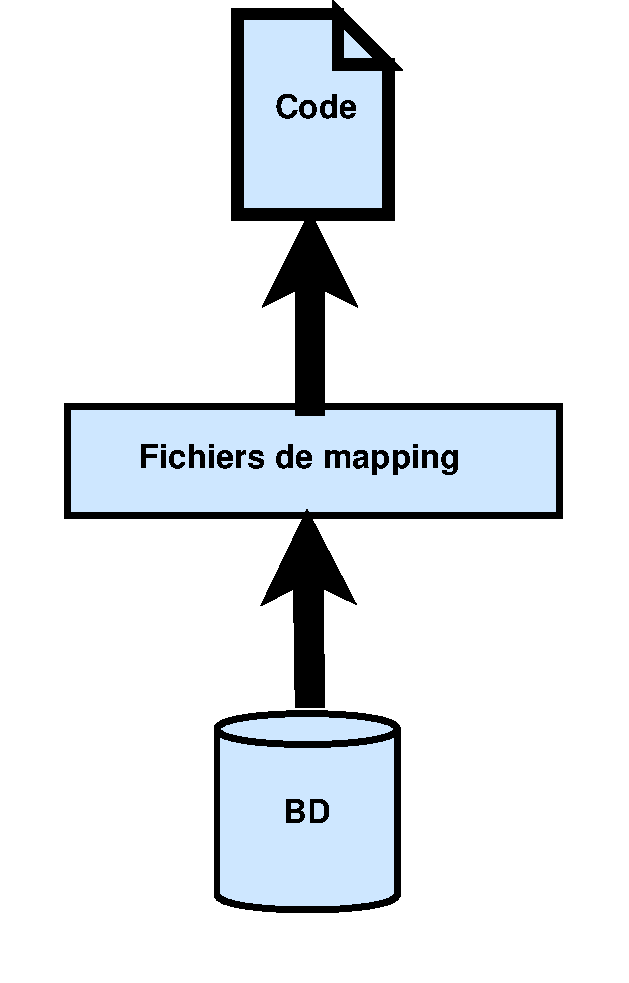
\includegraphics[scale=0.225]{images/bottomUp}
					\caption{Bottom Up}
				\end{center}
			\end{figure}
		\end{column}
	
	\end{columns}
	\end{block} 
\end{frame}



%%%%%%%%%%%%%%%%%%%%%%%%%%%%%%%%%%%%%%%%%%%%%%%%%%%

\speaker{\Julie}
\begin{frame}
	\frametitle{\underline{M}VC : Le modèle}
	\begin{block}{Top Down}
		Avantages :
		\begin{itemize}
			\item Approche objet
			\item Doctrine initialement prévu pour une approche top down
		\end{itemize}
 
		Inconvénients :
		\begin{itemize}
			\item Non visibilité du cycle de vie
			\item Création d'une table intermédiaire pour les attributs multivalués
			\item Mauvaise gestion de l'héritage
			\item Mauvaise gestion des attributs d'association
			
		\end{itemize}
	\end{block}
\end{frame}

%%%%%%%%%%%%%%%%%%%%%%%%%%%%%%%%%%%%%%%%%%%%%%%%%%%

\begin{frame}
	\frametitle{\underline{M}VC : Le modèle}
	\begin{block}{Bottom up}
	Avantages :
		\begin{itemize}
			\item Propreté de la Base de Données
			\item Amélioration des performances
			\item Vérification des contraintes dans la Base de Données
		\end{itemize} 
	Inconvénients :
		\begin{itemize}
			\item ORM non adapté
			\item Vérification et modifications d'une partie des fichiers générés
		\end{itemize}
	\end{block}
  
\end{frame}

%%%%%%%%%%%%%%%%%%%%%%%%%%%%%%%%%%%%%%%%%%%%%%%%%%%

\begin{frame}
	\frametitle{\underline{M}VC : Le modèle}
	\begin{block}{Décision : Bottom Up}
		\begin{itemize}
		\item Une bonne structure de base représente une anticipation des problèmes par la suite 
		\item Mieux adapté pour une possible utilisation au niveau Unicef France
		\end{itemize}
		
		
	\end{block}
\end{frame}